\documentclass[12pt,a4paper,fleqn]{article}
\usepackage{rmpackages}																% usual packages
\usepackage{rmtemplate}																% graphic charter
\usepackage{rmexocptce}																% for DS with cptce eval

%\cfoot{} 													% if no page number is needed
%\renewcommand\arraystretch{1.5}		% stretch table line height

\usepackage{fontawesome}
\newcommand{\thumbsup}{\marginpar{\faThumbsOUp}}

\begin{document}

\begin{header}
Activité -- À propos de la couleur des étoiles
\end{header}

\begin{multicols}{2}
\begin{center}
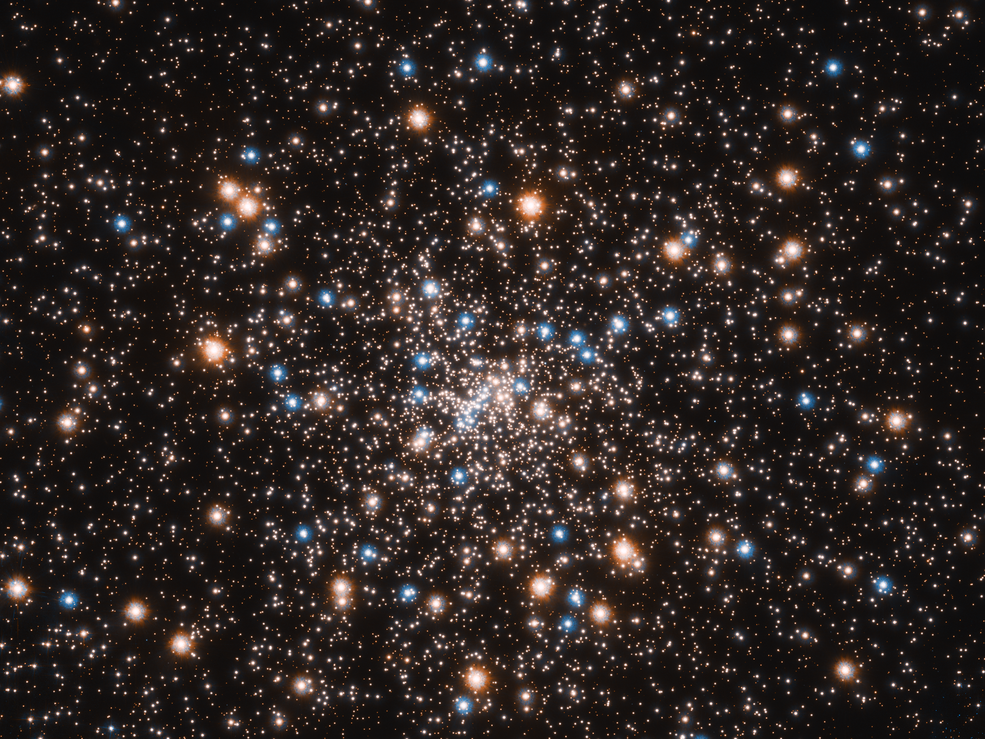
\includegraphics[trim=0 100 0 100, clip, width=\linewidth]{images/hubble_globular_cluster.png}
\end{center}

Comme le filament d'une ampoule ou une barre de métal chauffée à blanc, les étoiles sont des corps chauds (très chauds) qui émettent de la lumière.

On veut établir le lien entre la température d'une étoile et sa couleur, ce qui permet par exemple d'étudier précisément des étoiles pourtant situées très loin de nous.
\end{multicols}

On ne peut pas mesurer directement la température d'une étoile.
On va donc tout d'abord utiliser une lampe à incandescence dont on peut modifier la température du filament. 

\begin{enumerate}
\item \rea{}

Faire un schéma de l'expérience à réaliser pour obtenir le spectre du rayonnement de la lampe en utilisant une fente et un réseau.

\vspace{100pt}
\end{enumerate}

\begin{appel}
\rea{}
\end{appel}

Pour deux températures différentes, on observe les spectres ci-dessous :
\vspace{100pt}
\begin{enumerate}[resume]
\item \app{}

Comparer ces spectres.
Quelles sont leurs points communs ?
Leurs différences ?
\end{enumerate}

\begin{center}
\begin{tikzpicture}
\draw [color=white] (0,.5) -- ++ (.99\linewidth, 0);
\foreach \i in {0,1,...,4} {
  \draw [color=gray_c] (0,-.9*\i) -- ++ (.99\linewidth, 0);
}
\end{tikzpicture}
\end{center}

\begin{enumerate}[resume]
\item \anarai{}

Comment évolue la couleur de la radiation émise avec le maximum d'intensité en fonction de la température ?

\textit{Vous pouvez demander un spectre supplémentaire à une température plus élevée.} \thumbsup{}
\end{enumerate}

\begin{center}
\begin{tikzpicture}
\draw [color=white] (0,.5) -- ++ (.99\linewidth, 0);
\foreach \i in {0,1,...,2} {
  \draw [color=gray_c] (0,-.9*\i) -- ++ (.99\linewidth, 0);
}
\end{tikzpicture}
\end{center}

\section*{Température et couleur des étoiles}

Les images ci-dessous montrent la couleur et le spectre de quelques étoiles \og proches \fg{}.

\begin{center}
\newcommand{\localheight}{75 pt}
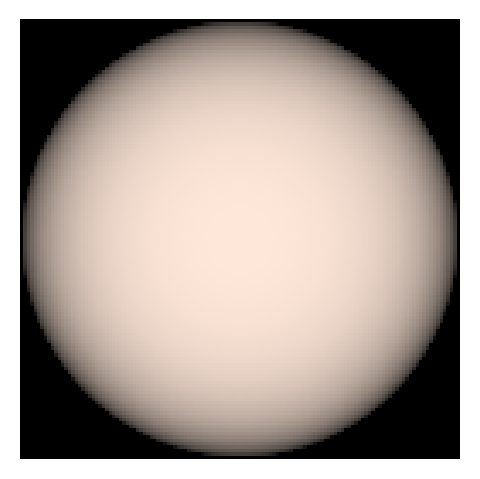
\includegraphics[height=\localheight]{images/star_sun.png}

\includegraphics[height=\localheight]{images/spectrum_star_sun.png}

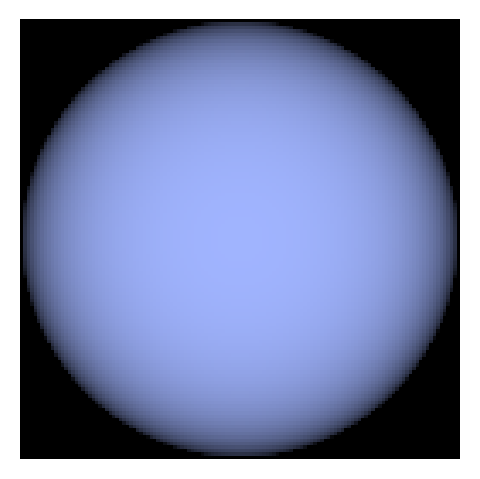
\includegraphics[height=\localheight]{images/star_rigel.png}

\includegraphics[height=\localheight]{images/spectrum_star_rigel.png}

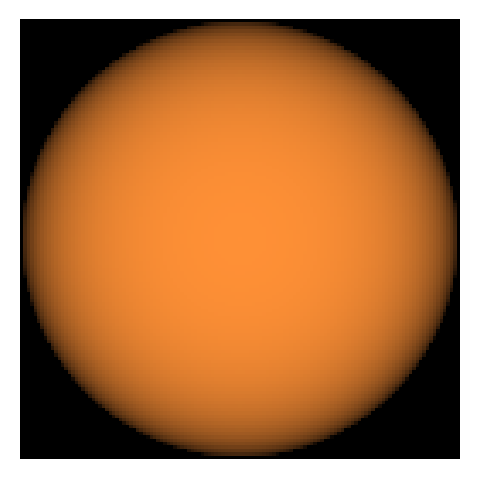
\includegraphics[height=\localheight]{images/star_proxima_centauri.png}

\includegraphics[height=\localheight]{images/spectrum_star_proxima_centauri.png}
\end{center}

\begin{enumerate}[resume]
\item \anarai{}

Classer ces étoiles de la plus froide à la plus chaude.

\textit{Si besoin, vous pouvez demander un coup de pouce.} \thumbsup
\end{enumerate}

\begin{center}
\begin{tikzpicture}
\draw [color=white] (0,.5) -- ++ (.99\linewidth, 0);
\draw [color=gray_c] (0,0) -- ++ (.99\linewidth, 0);
\end{tikzpicture}
\end{center}

\begin{enumerate}[resume]
\item \val{}

Ces observations confirment-elles votre hypothèse ?
\end{enumerate}

\begin{center}
\begin{tikzpicture}
\draw [color=white] (0,.5) -- ++ (.99\linewidth, 0);
\foreach \i in {0,1} {
  \draw [color=gray_c] (0,-.9*\i) -- ++ (.99\linewidth, 0);
}
\end{tikzpicture}
\end{center}
\vfill

\begin{appel}
\val{}
\end{appel}





\end{document}